\section{Finger Knuckle Project}
\subsection{Triplet Loss Function}
As for all model, I trained on the all samples of left middle finger knuckle, and then test on the rest fingers with all-to-all protocol. I also fit the RSIL on the SSIM index, called RSSSIM loss, which can get the best performance at present even on the little finger knuckle. Because the little finger knuckle can be more easily deform when compared to the rest ring, middle, and index finger knuckle. At the same time I also change the RFN model to output 64 channels feature map for getting more robust matching performance.

\begin{figure}[ht!]
    \centering
    \subfloat[]{
        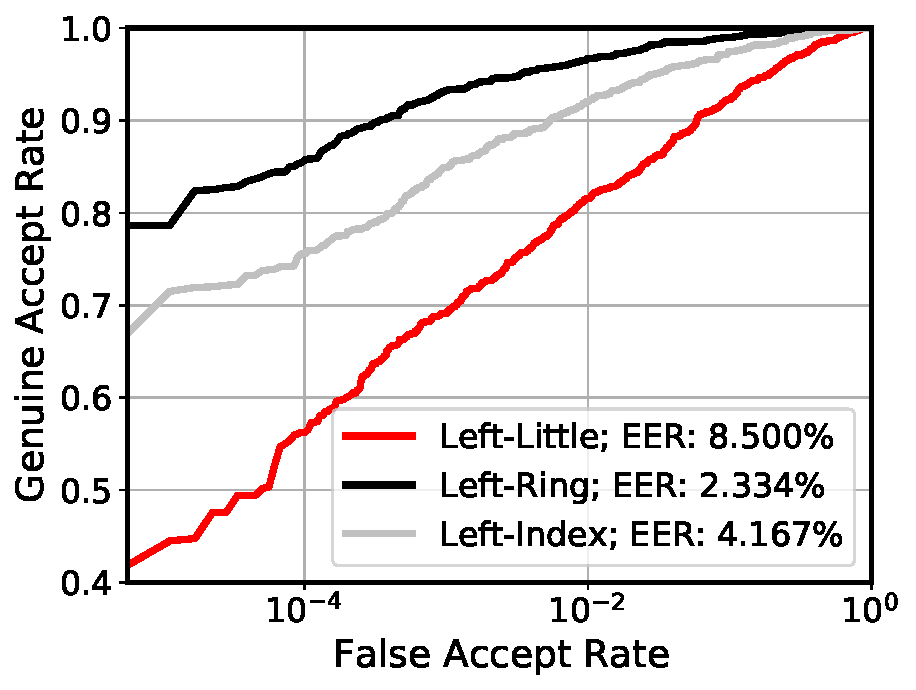
\includegraphics[width=2in]{Figure/02-12-2022/rfn-roc.pdf}
        \label{}
    }
    \subfloat[]{
        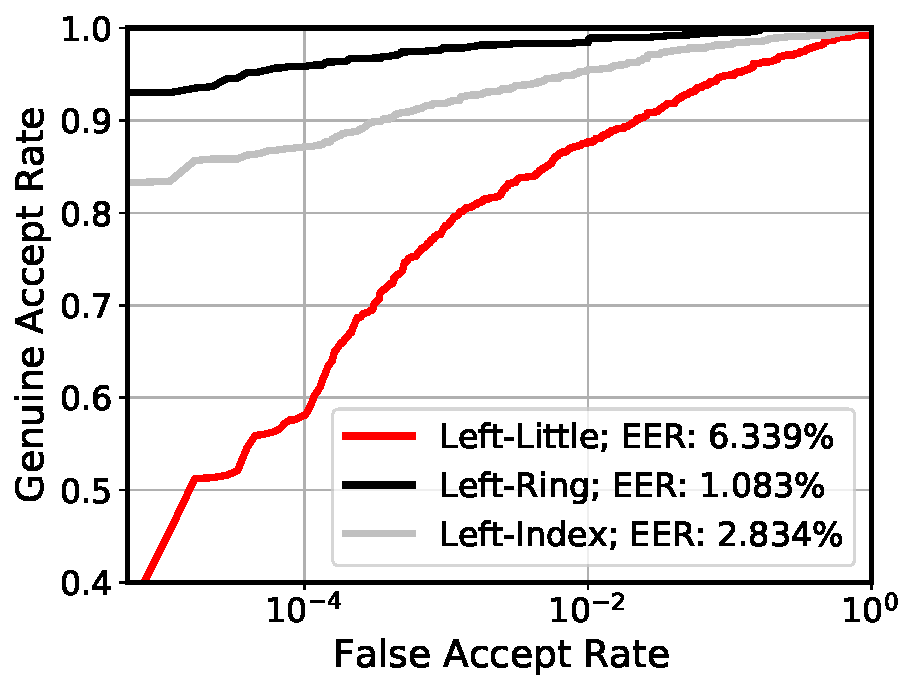
\includegraphics[width=2in]{Figure/02-12-2022/rfn-rsil-roc.pdf}
        \label{}
    }
    \subfloat[]{
        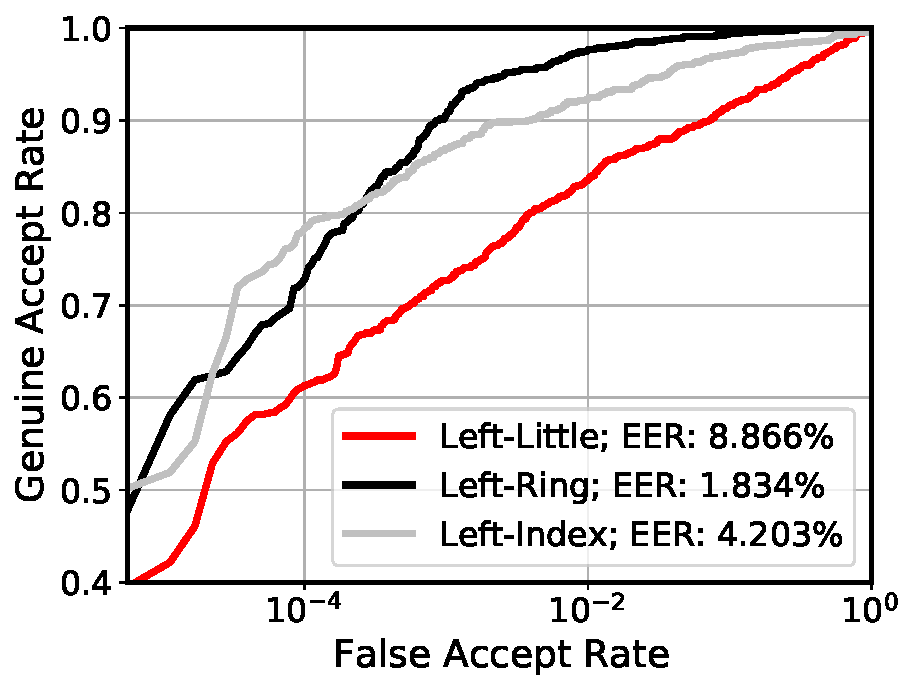
\includegraphics[width=2in]{Figure/02-12-2022/rfn-ssim-roc.pdf}
        \label{}
    }

    \subfloat[]{
        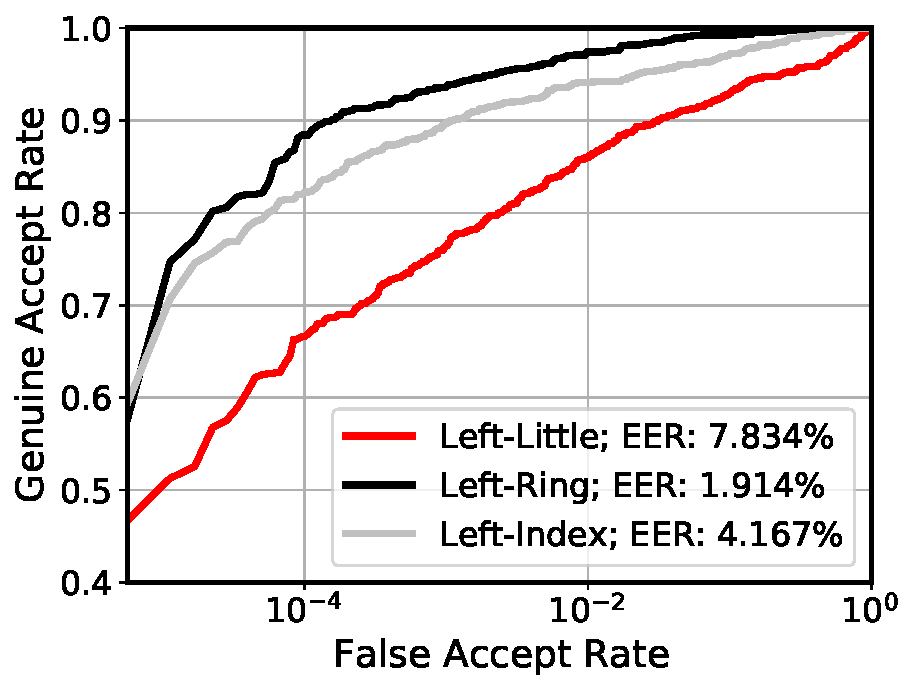
\includegraphics[width=2in]{Figure/02-12-2022/rfn64-ssim-roc.pdf}
        \label{}
    }
    \subfloat[]{
        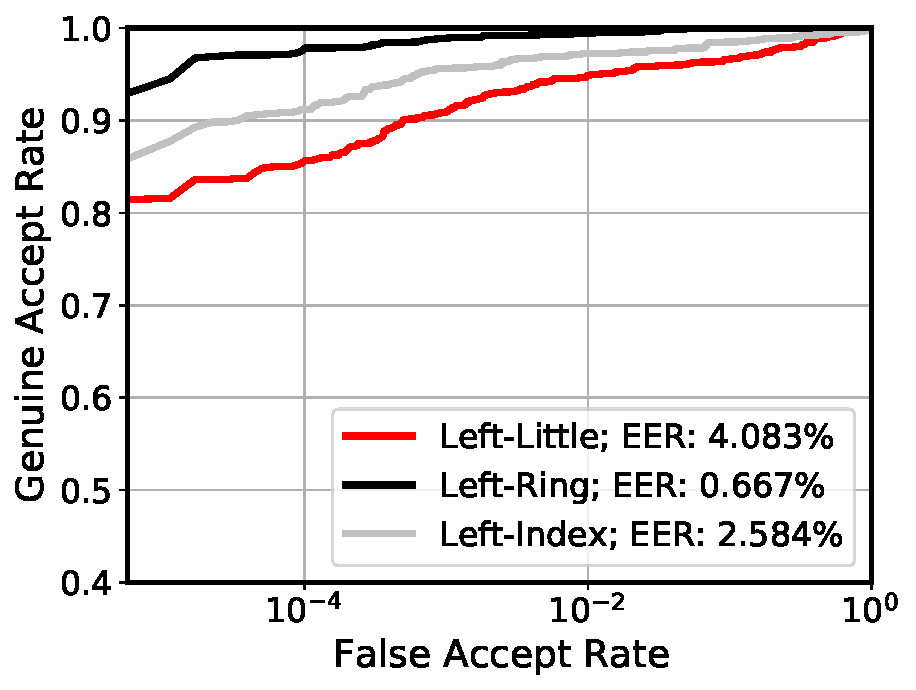
\includegraphics[width=2in]{Figure/02-12-2022/rfn64-rsssim-roc.pdf}
        \label{}
    }

    \caption{Comparative matching performance of different triplet loss function: (a) RFN-MSE; (b)RFN-RSIL; (c) RFN-SSIM; (d) RFN64-SSIM; (e) RFN64-RSSSIM}
    \label{triplet}
\end{figure}

\subsubsection{RFN64-RSSSIM}
RFN64-RSSSIM can get the best performance as shown on the Fig. \ref{triplet} when compared to other models. Therefore, I test the performance on the rest finger knuckle as shown on the ROC of Fig. \ref{rfn64-rssim}. And our performance also outperform the DON model on the Technical Report.
\begin{figure}[h]
    \centering
    \subfloat[]{
        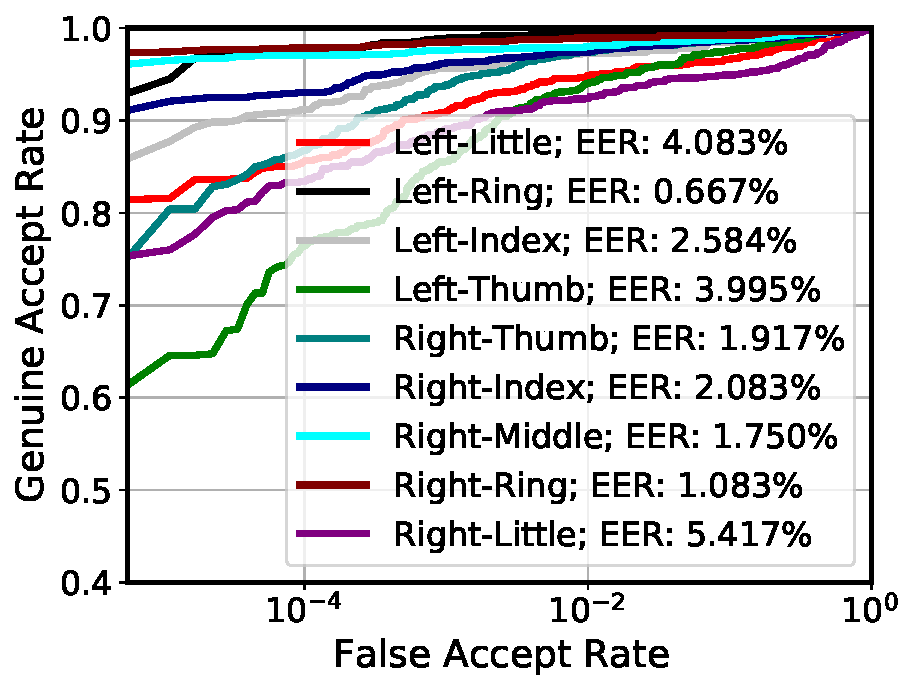
\includegraphics[width=4in]{Figure/02-12-2022/rfn64-rsssim-all-roc.pdf}
        \label{}
    }
    \caption{Comparative matching performance of RFN64-RSSIM model ROC cure.}
    \label{rfn64-rssim}
\end{figure}


\subsection{Score Fusion}
I fused the RFN64-RSSSIM (trained with triplet loss) finger knuckle matching scores and fingerprint matching scores using different method. As for different finger knuckle, the wight of fusion score can be different.
\subsubsection{Dynamic}

\begin{table}[h]
    \centering
    \caption{Dynamic score fusion}
    \begin{tabular}{lllllllll}
    \hline
        & \multicolumn{8}{c}{Finger Knuckle}                                    \\
        & 1      & 2      & 5      & 5      & 6      & 7      & 8      & 9      \\ \hline
    W   & 0.35   & 0.25   & 0.5    & 0.1    & 0.5    & 0.15   & 0.3    & 0.5    \\
    EER & 1.50\% & 0.57\% & 1.67\% & 0.50\% & 0.83\% & 0.33\% & 0.42\% & 0.58\% \\ \hline
    \end{tabular}
\end{table}

\subsubsection{Holistic}

\begin{table}[h]
    \centering
    \caption{Holistic score fusion}
    \begin{tabular}{lllllllll}
    \hline
        & \multicolumn{8}{c}{FInger Knuckle}                                    \\
        & 1      & 2      & 4      & 5      & 6      & 7      & 8      & 9      \\ \hline
    W   & 0.45   & 0.35   & 0.65   & 0.15   & 0.6    & 0.2    & 0.4    & 0.65   \\
    EER & 1.50\% & 0.57\% & 1.68\% & 0.50\% & 0.83\% & 0.33\% & 0.42\% & 0.66\% \\ \hline
    \end{tabular}
    \end{table}
\subsubsection{Nonlinear}

\begin{table}[h]
    \centering
    \caption{Nonlinear score fusion}
    \begin{tabular}{lllllllll}
    \hline
        & \multicolumn{8}{c}{Finger Knuckle}                                    \\
        & 1      & 2      & 4      & 5      & 6      & 7      & 8      & 9      \\ \hline
    W   & 0.55   & 0.45   & 0.9    & 0.15   & 0.85   & 0.25   & 0.5    & 0.9    \\
    EER & 1.50\% & 0.58\% & 1.70\% & 0.50\% & 0.91\% & 0.33\% & 0.42\% & 0.67\% \\ \hline
    \end{tabular}
    \end{table}

\subsection{Quadruplet Loss Function}
Then I trained RFN64-RSSSIM model with quadruplet loss function, the performance can clearly be shown on the Fig. \ref{quadruplet}. When can clearly get a conclusion that the quadruplet loss can increase the matching performance with slightly when compaed the Fig. \ref{quadruplet} a and c.

\begin{figure}[ht!]
    \centering
    \subfloat[]{
        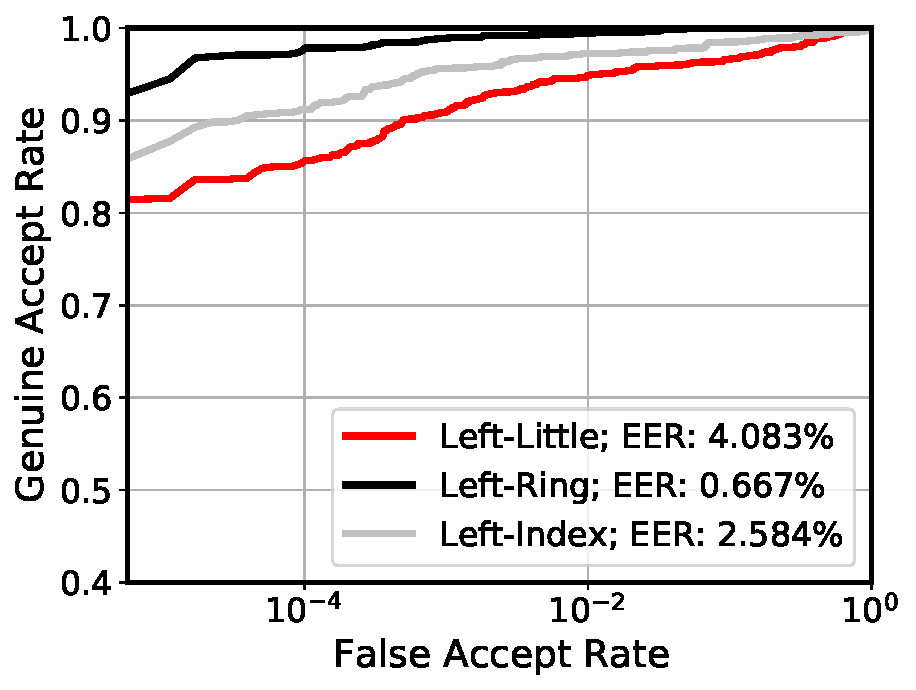
\includegraphics[width=2in]{Figure/02-12-2022/rfn64-rsssim-roc.pdf}
        \label{}
    }
    \subfloat[]{
        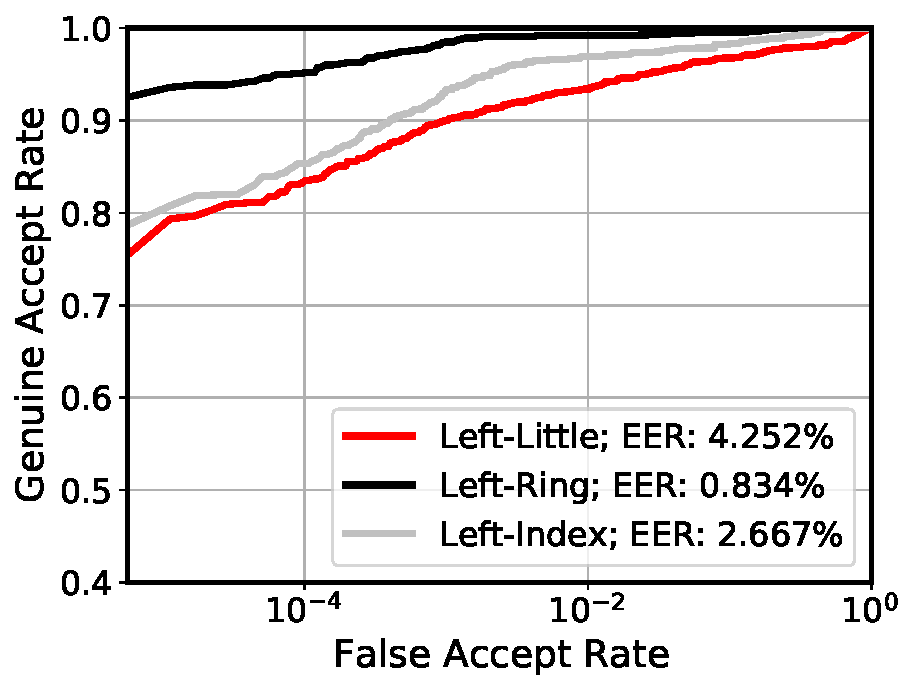
\includegraphics[width=2in]{Figure/02-12-2022/rfn64-rsssim-0.5-0.2-roc.pdf}
        \label{}
    }
    \subfloat[]{
        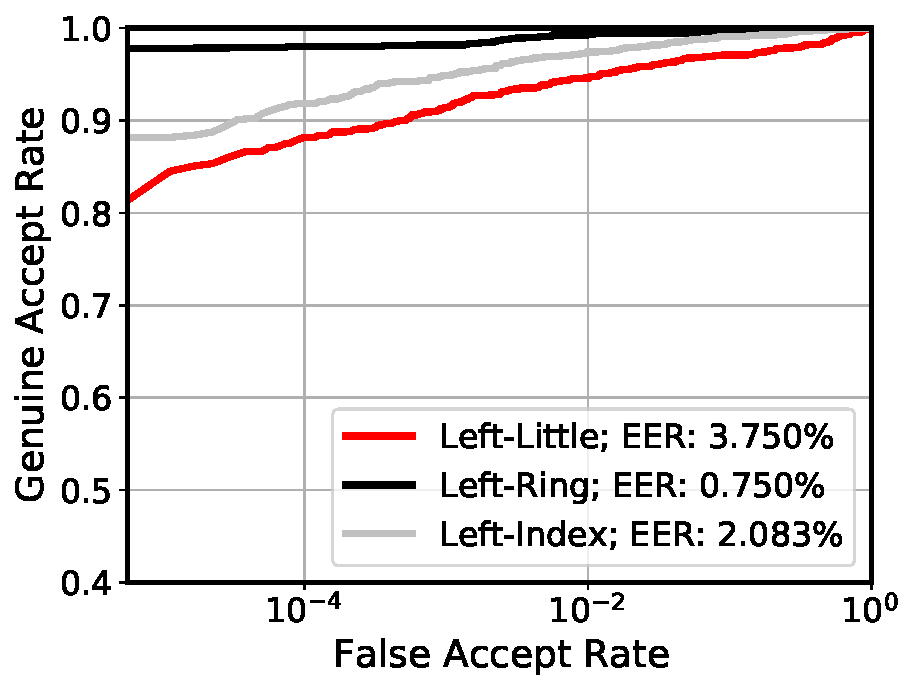
\includegraphics[width=2in]{Figure/02-12-2022/rfn64-rssim-0.5-0.3-roc.pdf}
        \label{}
    }

    \caption{Comparative matching performance wit quadruplet loss function: (a) triplet loss function; (b) $\alpha$1=0.5 and $\alpha$2=0.2; (c) $\alpha$1=0.5 and $\alpha$2=0.3}
    \label{quadruplet}
\end{figure}
